%!TEX program = xelatex.exe
\documentclass[14pt,a4paper]{article}
% \usepackage[pdftex,
%     pdfauthor={К.С.~Пилипенко},
%     pdfsubject={The Subject},
%     pdfkeywords={Первое ключевое слово, второе ключевое слово},
%     pdfproducer={LuaLatex with hyperref},
%     pdfcreator={Lualatex},
%     % hidelinks
% ]{hyperref}
%%%%%%%%%%%%%%Пользовательские команды%%%%%%%%%
\usepackage{calc}
\usepackage{color}
\usepackage{listing}
\usepackage{svg}
\usepackage{hhline}
\usepackage{multirow}
\usepackage{latexsym,amsmath,amssymb,amsbsy,graphicx}
\usepackage{listings}
\usepackage{icomma}
\usepackage[obeyspaces]{url} %Позволяет прописывать путь к файлам
\usepackage[american,siunitx]{circuitikz}
\def\centerarc[#1][#2](#3:#4:#5){\draw[#1]($(#2)+({#5*cos(#3)},{#5*sin(#3)})$)}
\usepackage[version=4]{mhchem} % the canonical chemistry package (example: \ce{^{32}_{15}P})
\usepackage{graphicx}
\usepackage{pgfplots}
\usepackage{wrapfig}
\graphicspath{{images/}}
\DeclareGraphicsExtensions{.pdf,.png,.jpg}
\usepackage{hyperref}
\hypersetup{
    colorlinks=true,
    linkcolor=blue,
    filecolor=magenta,      
    urlcolor=cyan,
    pdfauthor={К.С.~Пилипенко},
    pdfsubject={Основы обработки результатов исследования в физике},
    % pdfkeywords={Первое ключевое слово, второе ключевое слово},
    pdfproducer={LuaLatex with hyperref},
    pdfcreator={Lualatex},
    pdfpagemode=FullScreen,
    }
\urlstyle{same}
%Форматирование разделов
\usepackage{titlesec}
\usepackage{multicol} %Многоколоночный список
%%% Кастомизация разделов
\titleformat
{\section} % command
[block] % shape
{\normalfont\bfseries\itshape} % format
{Задание №\thesection.}{0.5em}{} % label
\newcommand{\progress}{\begin{center}\large\bfseries Ход работы\end{center}}
\newcommand{\questions}{\begin{center}\large\bfseries  Контрольные вопросы \end{center}}
%%%%%%%%%%%%%%%%%%%%%%%%Оформление по ГОСТУ
\usepackage{fontspec}
\setmainfont[Renderer=Basic,Ligatures={TeX}]{Times New Roman}
% \usepackage[english,russian]{babel} %Поддержка русской локализации
\setmonofont{dejavusansmono} % verbatim с кириллицей
\usepackage[14pt]{extsizes} % для того чтобы задать нестандартный 14-ый размер шрифта
\usepackage{indentfirst} %Задаёт отступ самого первого абзаца
\setlength\parindent{1.25cm}
\usepackage[a4paper, left=3cm, top=1.5cm, right=1.5cm, bottom=2cm]{geometry}
\usepackage{setspace}
\sloppy %Выравнивание текст по ширине и решение проблемы переполнением строки
\onehalfspacing %Полуторный интервал
%%%%%%%%%%%%%%%%%%%%%%%%%%%%% Добавление списка литературы
\usepackage{polyglossia}[2014/05/21]            % Поддержка многоязычности (fontspec подгружается автоматически)
\setmainlanguage[babelshorthands=true]{russian}  % Язык по-умолчанию русский с поддержкой приятных команд пакета babel
\setotherlanguage{english}                       % Дополнительный язык = английский (в американской вариации по-умолчанию)
\setmonofont{Courier New}
\newfontfamily\cyrillicfonttt{Courier New}
    \defaultfontfeatures{Ligatures=TeX,Mapping=tex-text}
\setmainfont{Times New Roman}
\newfontfamily\cyrillicfont{Times New Roman}
\setsansfont{Arial}
\newfontfamily\cyrillicfontsf{Arial}
\usepackage[
    bibencoding=utf8,% кодировка bib файла
    sorting=none,% настройка сортировки списка литературы
    style=gost-numeric,% стиль цитирования и библиографии (по ГОСТ)
    language=autobib,% получение языка из babel/polyglossia, default: autobib % если ставить autocite или auto, то цитаты в тексте с указанием страницы, получат указание страницы на языке оригинала
    autolang=other,% многоязычная библиография
    clearlang=true,% внутренний сброс поля language, если он совпадает с языком из babel/polyglossia
    defernumbers=true,% нумерация проставляется после двух компиляций, зато позволяет выцеплять библиографию по ключевым словам и нумеровать не из большего списка
    sortcites=true,% сортировать номера затекстовых ссылок при цитировании (если в квадратных скобках несколько ссылок, то отображаться будут отсортированно, а не абы как)
    doi=false,% Показывать или нет ссылки на DOI
    isbn=false,% Показывать или нет ISBN
]{biblatex}
\DeclareSourcemap{ %модификация bib файла перед тем, как им займётся biblatex 
    \maps{
        \map{% перекидываем значения полей language в поля langid, которыми пользуется biblatex
            \step[fieldsource=language, fieldset=langid, origfieldval, final]
            \step[fieldset=language, null]
        }
    }
}
\emergencystretch=1em
\addbibresource{literature.bib}
%%%%%%%%%%%%%%%%%%%%%%%%
\author{\href{mailto:www-kirill.pilipenko@yandex.ru}{К.С.~Пилипенко} \href{https://github.com/PilipenkoKirill/MeasurementLabs}{
\includegraphics[width=.5cm]{images/gitHubLogo.pdf}}} %Через \and можно добавить ещё авторов
\date{\the\year{}}

\title{Лабораторная работа №5 \\ \textit{Использования метода наименьших квадратов для аппроксимации результатов совместных измерений}}
\begin{document}
\maketitle
Пусть имеется два набора экспериментальных данных: $x_{i}$ и $y_{i}$, где ${i=1,...n}$\footnote{$n$~---~в данном случае это объёмом выборочных совокупностей} такие что между ними предполагается зависимость вида $y = f(x)$. 
Вводится некоторая (в простейшем случае линейная) функция $f(x, \{a_j\})$, которая определяется множеством неизвестных параметров $\{a_j\}$, где $j={1,...n}$.

Ставится задача получить такое множество, чтобы совокупность погрешностей $r_i=y_i-f(x_i, \{a_j\})$ была в некотором смысле минимальной.

Согласно методу наименьших квадратов решением этой задачи является набор параметров $\{a_i\}$, который минимизирует некоторую функцию:
\begin{equation} \label{leastSquares}
    g(\{a_i\}) = \sum\limits^n_{i=0} (y_i-f(x_i, \{a_j\}))^2.
\end{equation}

Пусть между данными предположительно имеется линейная зависимость, тогда $\{a_j\} = \{a_1,a_2\}$, а функция $f(x, a_1, a_2) = a_1x + a_2$. Чтобы функция $g(a_1,a_2)$ из уравнения \ref{leastSquares} была минимальна достаточным условием является равенство нулю её частных производных:
\begin{equation}
    \begin{cases}
        \left (\frac{\partial g(a_1,a_2)}{\partial a_1} \right )_{a_2} = 0 \\
        \left (\frac{\partial g(a_1,a_2)}{\partial a_2} \right )_{a_1} = 0
    \end{cases},
\end{equation}
где $\left (\frac{\partial g(a_1,a_2)}{\partial a_1} \right )_{a_2}$~---~производная функции по $a_1$ при постоянной $a_2$.

\progress{}
\section{Генерация выборки}
\noindent\begin{itemize}
	% \item Сгенерируйте выборку с помощью программы \texttt{NormDistGen.exe}. После запуска программы в той же папке появится новый файл;
	\item Создайте файл с расширением \texttt{.xlsm}. По умолчанию вкладка \texttt{Разработчик} спрятана, поэтому надо её включить. Заходим по пути \texttt{Файл$\rightarrow$Параметры$\rightarrow$Настроить ленту} и ставим галочку на вкладке \texttt{Разработчик};
	\item В разделе \texttt{Разработчик} нажмите на \texttt{макросы}, дайте любое название макроса и создайте его. Далее в открывшемся окне введите код из листинга \ref{SqDistGen};
	\lstset{ %
	language=[Visual]Basic,
	keywordstyle=\color{brown},          % Стиль ключевых слов
	breaklines=true,
	commentstyle=\color{gray}, % white comments
	numbers=left, 
	backgroundcolor=\color{lightgray!5!white},
	tabsize=4,
	texcl=true
	} 
	\begin{lstlisting} 
	Sub LinDistGen()
		' Сюда надо поместить код из листинга
	End Sub  
	\end{lstlisting}
	\item При запуске кода в первом и втором столбцах таблицы появится сгенерированные выборки $x_i$ и $y_i$ соответственно объёмом 50 элементов.
\end{itemize}
\section{Ручной поиск параметров} \label{manualMethod}
Аппроксимировать полученную зависимость будем линейной функцией вида $f(x,a_1,a_2) = a_1x + a_2$.
\begin{enumerate}
    \item Подставив $f(x,a_1,a_2)$ в формулу \ref{leastSquares} найдите частные производные\footnote{Более подробно о МНК можно узнать в учебнике \cite{Stepanova2014} на стр. 45}. В Excel можно и нужно производить расчёты таких коэффициентов как $\sum x_i, \sum x_i^2, \sum x_iy_i$ и т.п. \textbf{Получение частных производных и их дальнейшее упрощение нужно записывать в тетрадке!}
    \item Решите полученную систему линейных уравнений. Запишите полученный результат ($a_1$ и $a_2$) в отдельных ячейках таблицы Excel.
\end{enumerate}
\section{Машинный поиск параметров}
\begin{enumerate}
	\item Постройте график $y = f(x)$.
	\item Добавьте линейную линию тренда на графике и зайдите в \texttt{Дополнительные параметры} как показано на скриншоте.\\
	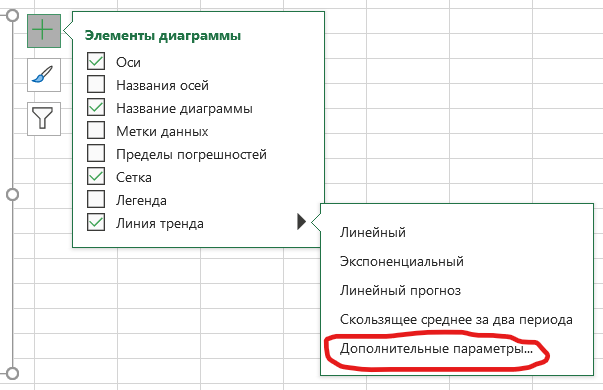
\includegraphics[width=.7\textwidth]{trendLine}
	\item В открывшейся панели поставьте галочку рядом с \texttt{показывать уравнение на диаграмме}.
	\item Сравните значения параметров $a_1$ и $a_2$ с полученными первым способом. Сделайте вывод.
\end{enumerate}

\questions{}
\begin{enumerate}
	\item Что представляет собой метод минимума хи-квадрат (метод Пирсона) и чем он отличается от МНК?
	\item В чём заключается метод максимального правдоподобия? % Метод заключается в оценивании неизвестного параметра путём максимизации функции правдоподобия
\end{enumerate}

\printbibliography[title={Литература}]	
\begin{center}
	\textbf{\Large Приложение}
\end{center}
\lstset{ %
	language=[Visual]Basic,
	keywordstyle=\color{brown},          % Стиль ключевых слов
	breaklines=true,
	numbers=left, 
	backgroundcolor=\color{lightgray!5!white},
	tabsize=4,
	label=SqDistGen, 
	caption={Код генератора выборки}
	} 
	\renewcommand{\lstlistingname}{Листинг}
\begin{lstlisting}
	Randomize
	Dim i As Long
	Dim a As Double
	Dim b As Double
	Dim c As Double
	Dim Error As Double
	Dim random As Double

	a = 2 * (2 * Rnd - 1)
	b = 3 * (2 * Rnd - 1)
	c = 2 * (2 * Rnd - 1)
	Error = 0.2
	i = 51
	Range("A1").Select
	For i = 2 To i
		ActiveCell.Value = i
		ActiveCell.Offset(0, 1).Select
		random = a * i * i + b * i + c
		ActiveCell.Value = random * (1 - Error + 2 * Error * Rnd)
		ActiveCell.Offset(1, -1).Select
	Next i
	\end{lstlisting}
\end{document}